\documentclass{article}
\usepackage[utf8]{inputenc}
\usepackage{graphicx}
\usepackage{titling}
\usepackage{amsmath}
\usepackage{amssymb}
\usepackage{cite}
\usepackage{hyperref}
\usepackage{float}
\usepackage{listings}
\usepackage{booktabs}
\usepackage[table]{xcolor}
\usepackage{geometry}
\usepackage{tikz}
\usetikzlibrary{shapes.geometric, arrows, positioning, fit, calc, shadows}
\usepackage{tcolorbox}
\tcbuselibrary{skins}
\usepackage{enumitem}
\usepackage{fancyhdr}
\usepackage{pagecolor}
\usepackage{tabularx}
\usepackage{svg}
\usepackage{xcolor}

% --- ARABIC SUPPORT ---
\usepackage{arabtex}
\usepackage{utf8}
\setcode{utf8}

% --- COLOR PALETTE (High Contrast Optimized) ---
\definecolor{primarybg}{RGB}{20, 20, 20} 
\definecolor{secondarygrey}{RGB}{129, 130, 131}
\definecolor{neutraltext}{RGB}{235, 235, 230} 
\definecolor{accentred}{RGB}{60, 170, 100}
% \definecolor{accentred}{RGB}{185, 60, 60} 
\definecolor{accentgold}{RGB}{210, 190, 120} 
\definecolor{boxbg}{RGB}{35, 35, 35} 

% Setup page geometry
\geometry{a4paper, margin=0.8in, bottom=1in}

% --- GLOBAL THEME SETUP ---
\pagecolor{primarybg}
\color{neutraltext}

% Setup headers and footers
\pagestyle{fancy}
\fancyhf{}
\renewcommand{\headrulewidth}{1pt}
\renewcommand{\footrulewidth}{1pt}
\renewcommand{\headrule}{\hbox to\headwidth{\color{accentred}\leaders\hrule height \headrulewidth\hfill}}
\renewcommand{\footrule}{\hbox to\headwidth{\color{accentred}\leaders\hrule height \footrulewidth\hfill}}


\fancyhead[L]{\textcolor{accentred}{\textbf{Baligh}}}
\fancyhead[R]{\textcolor{secondarygrey}{Document of Deliverables}}
\fancyfoot[C]{\textcolor{accentgold}{\thepage}}

% Custom box styles
\tcbset{
    mainbox/.style={
        enhanced,
        colback=boxbg,
        colframe=accentred,
        coltext=neutraltext,
        boxrule=1pt,
        arc=3mm,
        fonttitle=\bfseries\large,
        title style={fill=accentred, text=white},
        drop shadow
    },
    quotebox/.style={
        colback=primarybg,
        colframe=accentgold,
        coltext=neutraltext,
        boxrule=0pt,
        leftrule=3mm,
        arc=2mm,
        fontupper=\itshape
    }
}

\begin{document}

% --- TITLE PAGE (Original Template Style) ---
\begin{titlepage}
    \begin{center}
        \begin{minipage}[c]{0.12\textwidth}
            % Ensure these images exist in your project folder!
            
\includegraphics[width=\textwidth]{Cairo_University_Crest.png}
        \end{minipage}
        \hfill
        \begin{minipage}[c]{0.6\textwidth}
            \centering
            {\large Cairo University - Faculty Of Engineering \\ Computer Engineering Department \\ Graduation Project - Fall 2025 \par}
        \end{minipage}
        \hfill
        \begin{minipage}[c]{0.15\textwidth}
            
\includegraphics[width=\textwidth]{cairo-no-back.png}
        \end{minipage}
    \end{center}

    \noindent{\color{accentred}\hrulefill}

    % --- LOGO SPACE ---
    \begin{center}
        
\includegraphics[width=8cm]{baligh-transparent.png} 
    \end{center}
    % ------------------

    \begin{center}
        % Title Box: Black fill, Red border (Original Style)
        \tikz\node[draw=accentred, line width=1mm, fill=boxbg, inner sep=1cm, rounded corners=1cm]{\parbox{0.8\textwidth}{
                \centering
                \vspace{0.5cm}
                {\fontsize{32}{38}\selectfont \textcolor{accentgold}{\textbf{Document of Deliverables}} \par}
                \vspace{0.5cm}
                {\large Baligh: Arabic Writing Assistant\par}
                \vspace{0.5cm}
        }};
    \end{center}

    \begin{center}
    {\large Supervised by\par}
    {\Large \textbf{\textcolor{accentred}{Dr. Ayman AboElhassan}} \par}
    
    \vspace{1cm}

    \begin{tcolorbox}[mainbox, title=\textcolor{white}{Team Contact Information}, sharp corners=north, sharp corners=south]
        \renewcommand{\arraystretch}{1.2}
        \begin{tabularx}{\textwidth}{Xr}
            \textbf{\textcolor{accentgold}{Name}} & \textbf{\textcolor{accentgold}{Email}} \\
            \midrule
            \textcolor{white}{Ahmed Hamed Gaber Hamed} & \textcolor{secondarygrey}{ahmed.hamed03@eng-st.cu.edu.eg} \\
            \textcolor{white}{Akram Hany Karam Salam} & \textcolor{secondarygrey}{akram.sallam03@eng-st.cu.edu.eg} \\
            \textcolor{white}{Amir Anwar Bekhit Awd Kedis} & \textcolor{secondarygrey}{amir.awd03@eng-st.cu.edu.eg} \\
            \textcolor{white}{Somia Saad Ismail El-Shemy} & \textcolor{secondarygrey}{somia.elshemy02@eng-st.cu.edu.eg} \\
        \end{tabularx}
    \end{tcolorbox}
\end{center}

\begin{center}
    \vspace{1cm}
    {\large \today \par}
\end{center}

    \vfill
\end{titlepage}

\newpage
% Reset page number for content
\setcounter{page}{1}

% --- TEAM EMAILS (Required by Proposal Format) ---


% --- 1. PROBLEM STATEMENT ---
\section{\textcolor{accentred}{Problem Statement}}
While English speakers enjoy seamless writing assistants, Arabic users lack tools that have Grammatical Error Correction and Next-Word Suggestion with high accuracy and without significant input latency.

% --- 2. MOTIVATION ---
\section{\textcolor{accentred}{Motivation}}
We aim to build a high-quality MSA writing assistant that achieves SOTA accuracy with real-time performance, bridging the gap between current research advancements and available practical tools.

% --- 3. SYSTEM ARCHITECTURE ---
\section{\textcolor{accentred}{System Architecture}}

\begin{figure}[H]
    \centering
    
    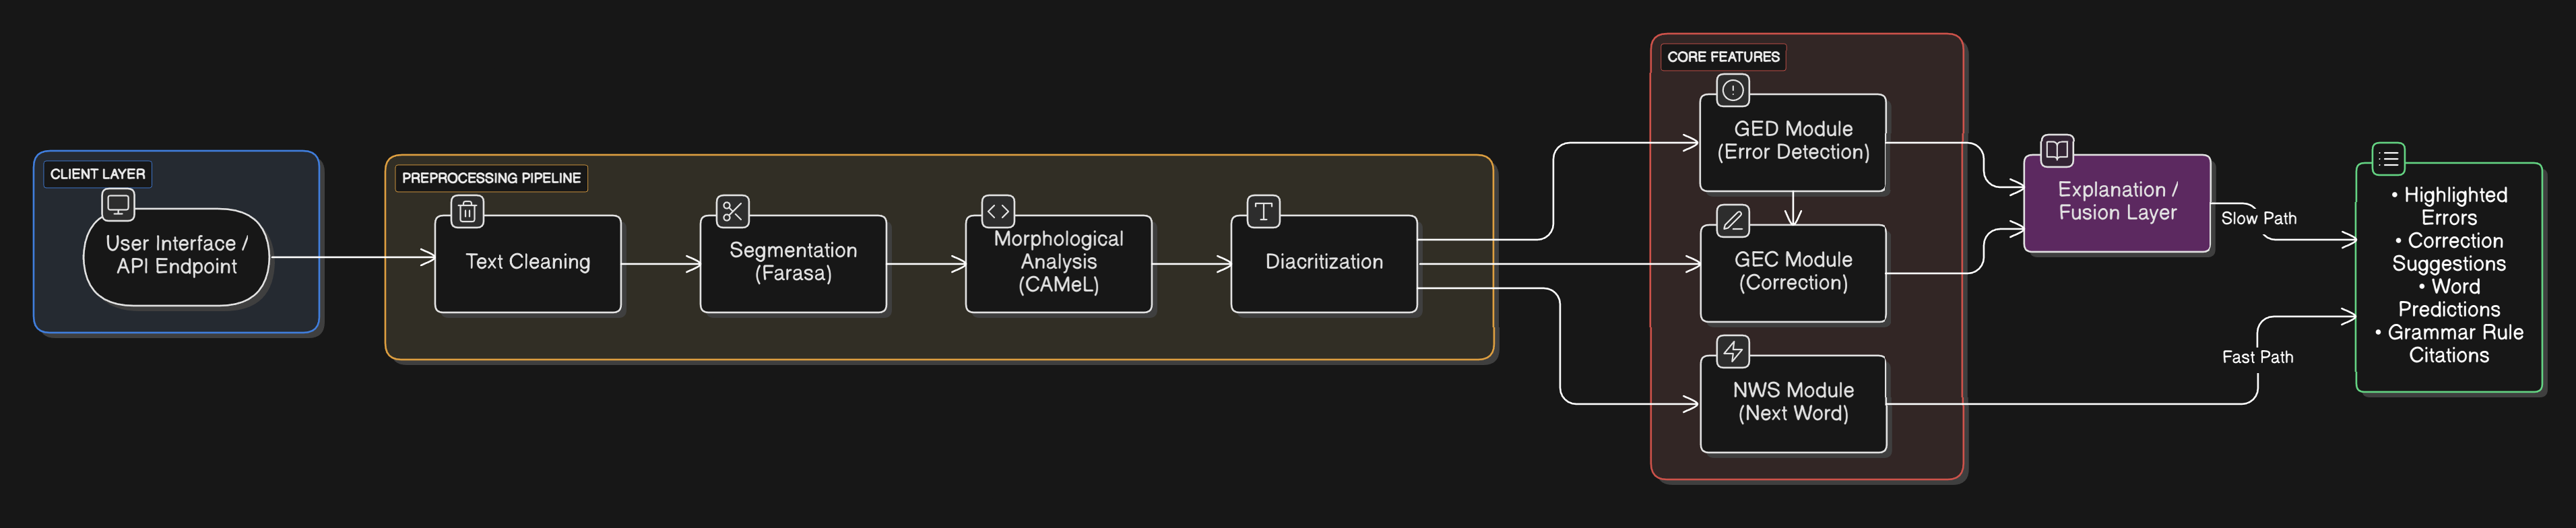
\includegraphics[width=\textwidth]{HL-Arch.png} % <-- UNCOMMENT THIS and remove tikzpicture when ready
    
    \caption{High-Level System Architecture of Baligh}
    \label{fig:architecture}
\end{figure}

\begin{figure}[H]
    \centering
    
    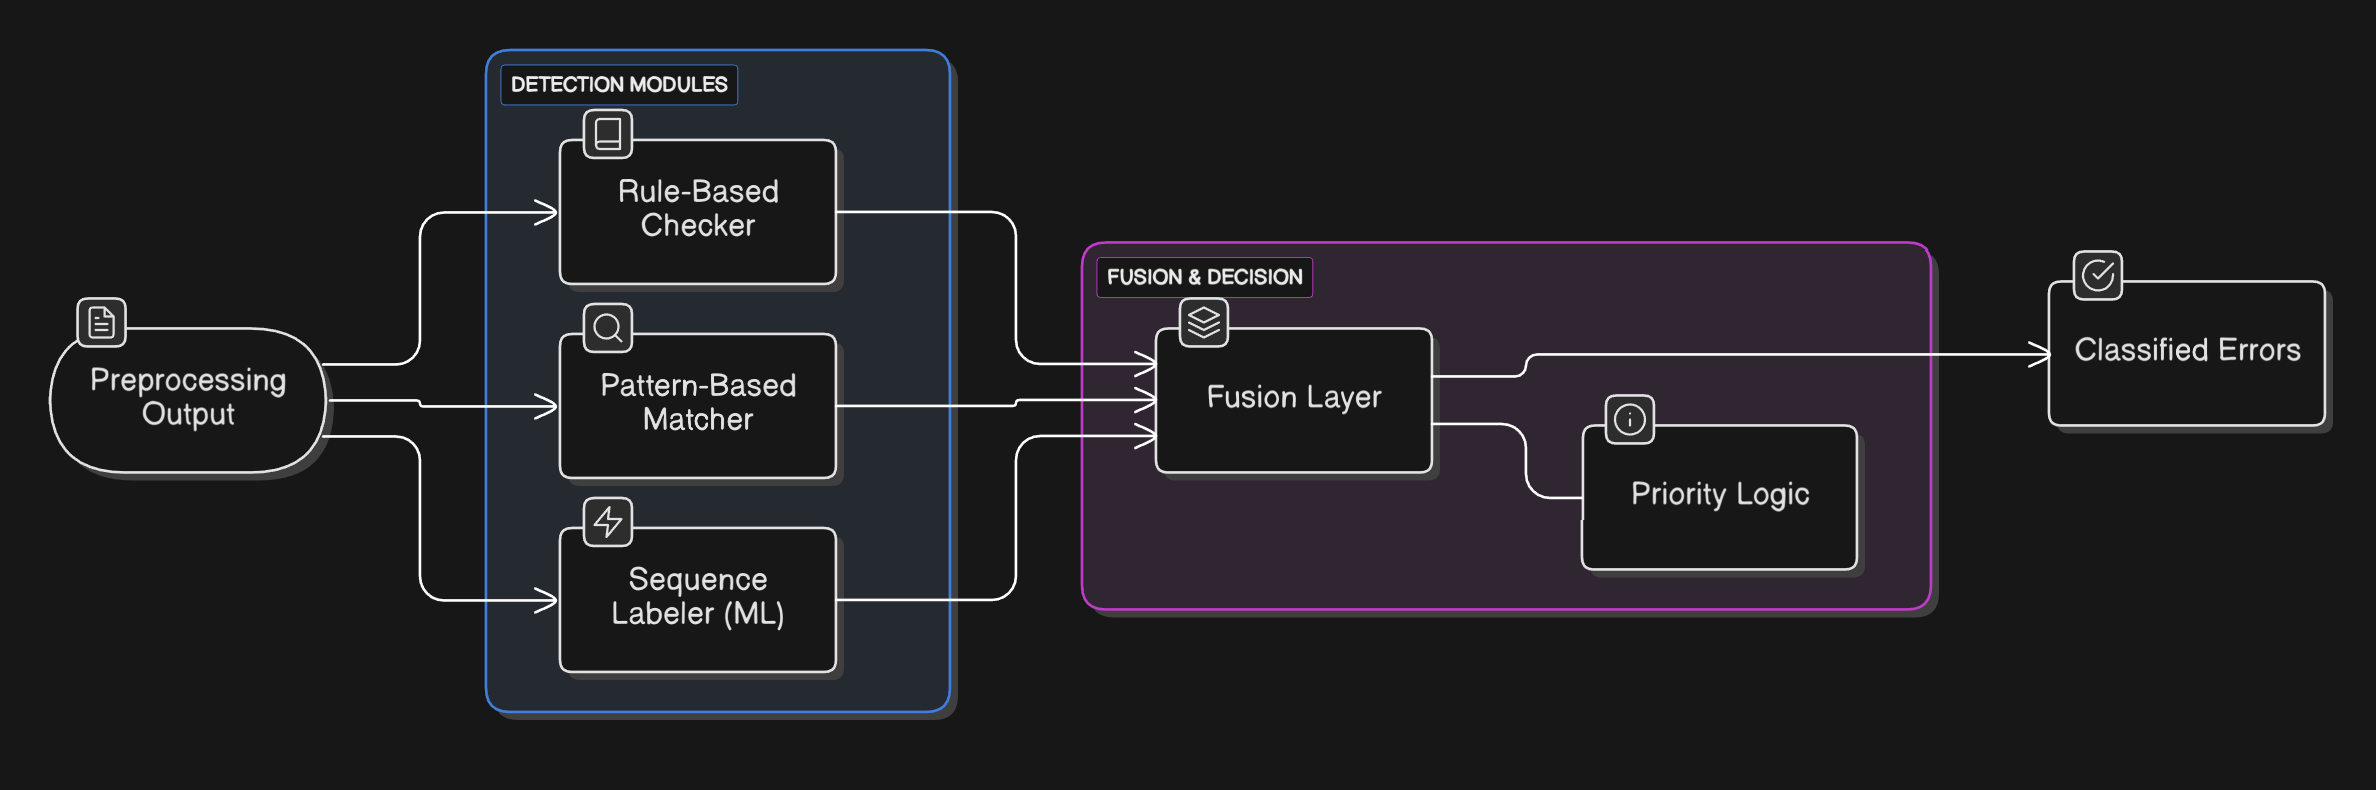
\includegraphics[width=\textwidth]{GED-diagram.png} % <-- UNCOMMENT THIS and remove tikzpicture when ready
    
    \caption{Grammatical Error Detection Architecture}
    \label{fig:architecture}
\end{figure}

\begin{figure}[H]
    \centering
    
    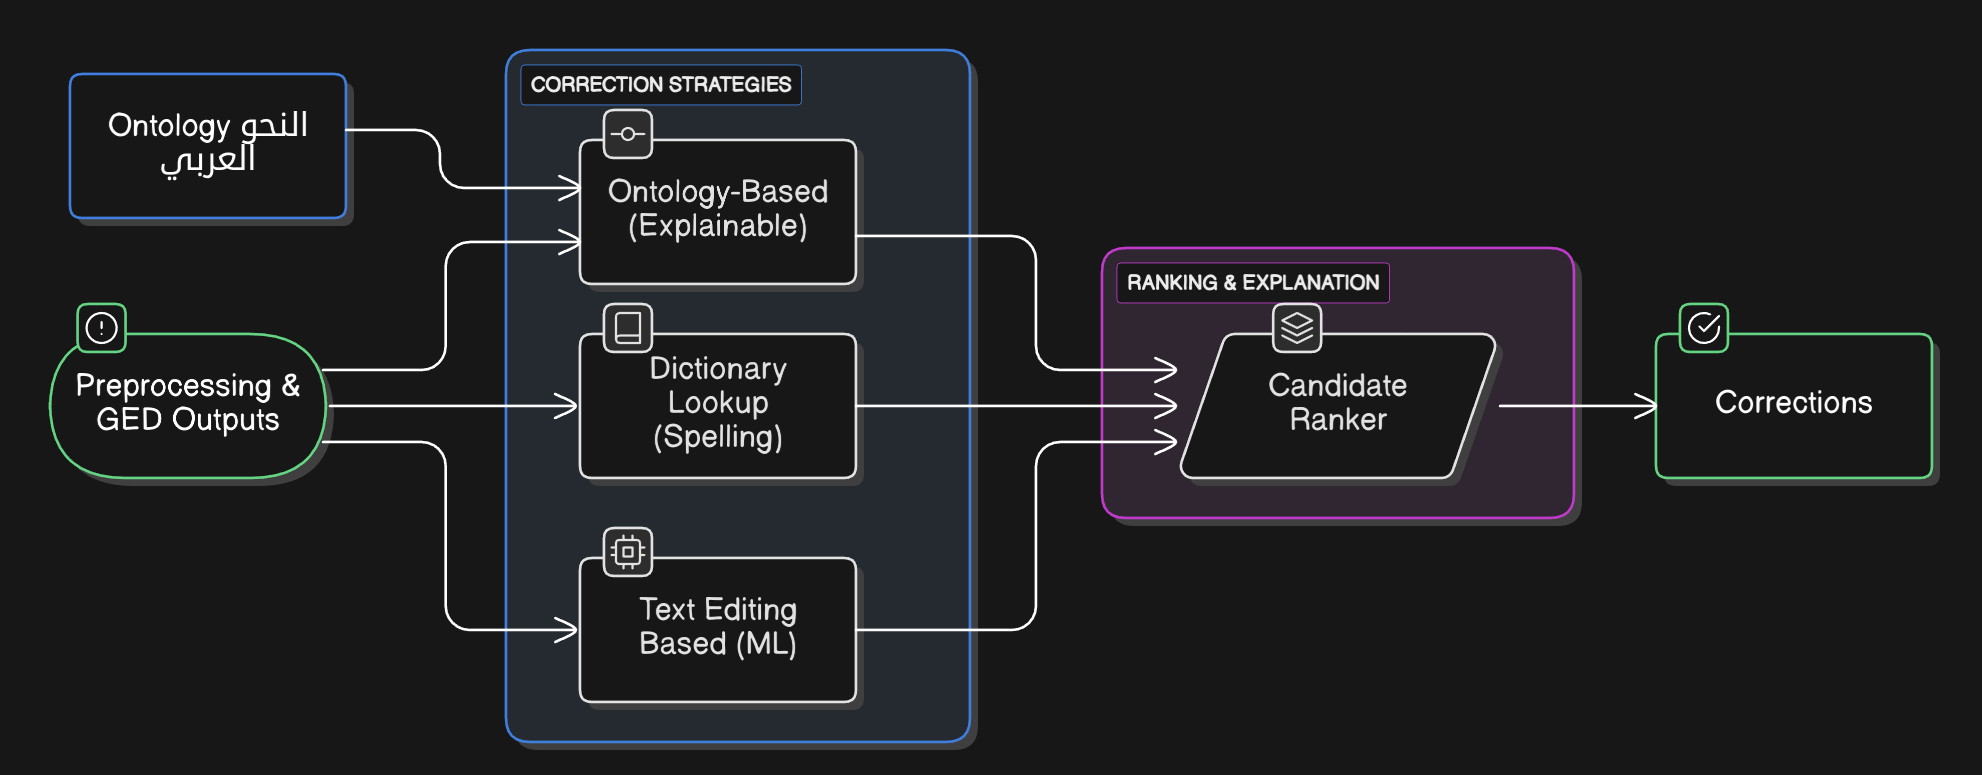
\includegraphics[width=\textwidth]{GEC-Arch_cl.png} % <-- UNCOMMENT THIS and remove tikzpicture when ready
    
    \caption{Grammatical Error Correction Architecture}
    \label{fig:architecture}
\end{figure}

\begin{figure}[H]
    \centering
        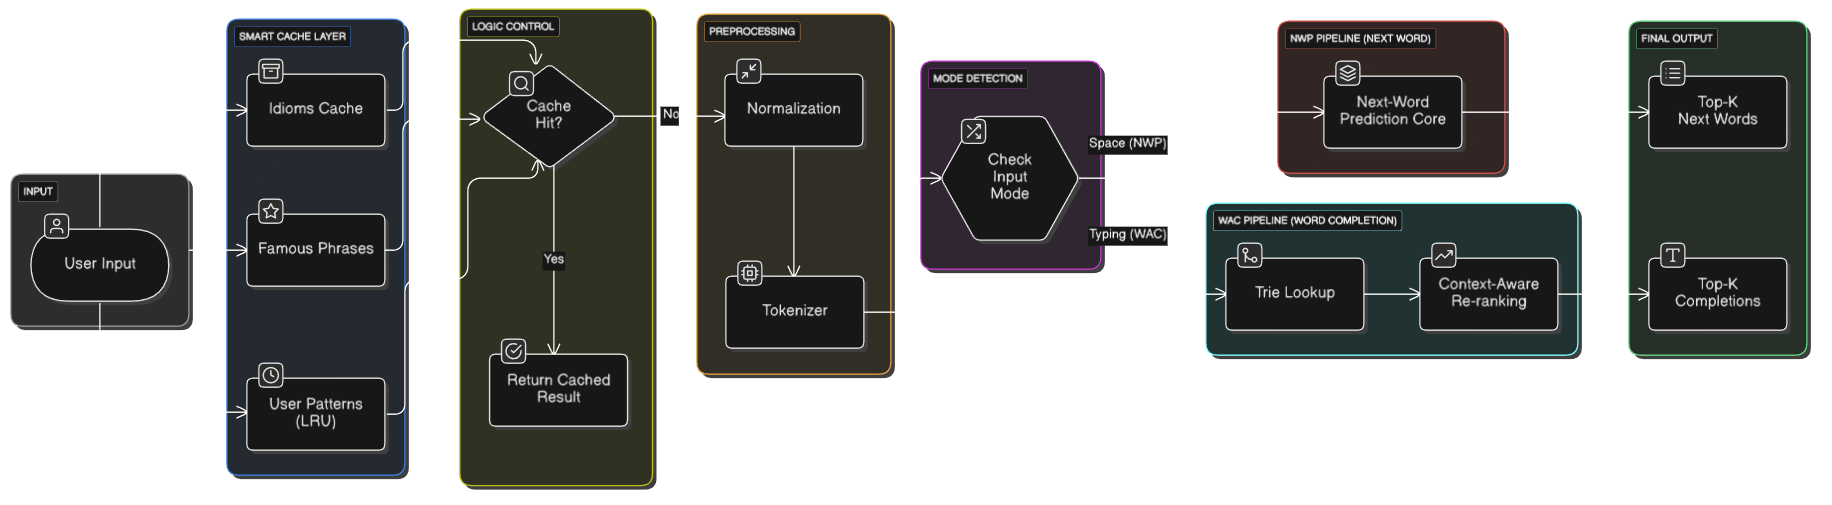
\includegraphics[width=\textwidth]{NWS.png} % <-- UNCOMMENT THIS and remove tikzpicture when ready

    
    \caption{Next Word Suggestion Architecture}
    \label{fig:architecture}
\end{figure}


% --- 4. DELIVERABLES ---
\section{\textcolor{accentred}{List of Deliverables}}

\begin{table}[H]
\centering
\footnotesize 
\renewcommand{\arraystretch}{1.8} 
\setlength{\tabcolsep}{8pt}       

% Start alternating colors from the 2nd row (leaving header alone)
% Row 2 gets primarybg, Row 3 gets boxbg, and so on.
\rowcolors{2}{primarybg}{boxbg}

\begin{tabularx}{\textwidth}{
    >{\raggedright\arraybackslash}p{3cm} 
    >{\raggedright\arraybackslash}X 
    >{\raggedright\arraybackslash}p{3cm} 
    >{\raggedright\arraybackslash}p{3.1cm} 
    c
}
% No top border

% Header Row (Manual Color overrides rowcolors)
\rowcolor{accentred} 
\textcolor{white}{\textbf{Module Name}} & 
\textcolor{white}{\textbf{Function}} & 
\textcolor{white}{\textbf{Input}} & 
\textcolor{white}{\textbf{Expected Output}} & 
\textcolor{white}{\textbf{\% Libs}} \\ 

% Module 1
\textbf{\textcolor{accentgold}{1. Preprocessing Module}} & 
Text cleaning, normalization, tokenization, and morphological analysis & 
User Input (Raw Arabic Text) & 
Tokenized text + Morphological Features (POS, SP, Lemma) & 
10\% \\ 
 

% Module 3
\textbf{\textcolor{accentgold}{2. GED Engine}} & 
Error Detection (Rules + Patterns + ML + Fusion) & 
Preprocessed Input & 
Final error list with confidence \& explanations & 
20\% \\ 

% Module 4
\textbf{\textcolor{accentgold}{3. GEC (Ontology \& Dictionary-Based)}} & 
Generate corrections using grammar ontology and spelling mistakes using dictionary & 
Preprocessed Input & 
Correction candidates & 
20\% \\ 

% Module 5
\textbf{\textcolor{accentgold}{4. GEC (Text Editing \& Ranking)}} & 
Text editing approach + candidate ranking + explanation generation & 
Preprocessed Input + M4 Correction Candidates & 
Final ranked corrections with explanations & 
15\% \\ 


% Module 2
\textbf{\textcolor{accentgold}{5. NWS Module}} & 
Next Word Suggestion & 
Preprocessed Input & 
Ranked list of predicted words & 
30\% \\

% Module 6
\textbf{\textcolor{accentgold}{6. API \& GUI}} & 
REST API + Frontend & 
User Inputs + All Modules Outputs & 
Web UI with a live text editor + (Optional Browser Extension) & 
20\% \\ 

% No bottom border
\end{tabularx}
\end{table}
\end{document}